\chapter{Имитационные модели оценки американского опциона}

Традиционный подход предполагает следование гипотезе эффективного рынка, которая влечёт определение <<справедливой>> цены опциона как \emph{такой цены, при которой ни продавец, ни покупатель в среднем не получают прибыли}. Тогда ценой Американского опциона является математическое ожидание прибыли, полученной при исполнении опциона в оптимальный момент времени, а задача оценки оказывается частным случаем проблемы остановки выбора (подробнее о проблеме с этой точки зрения можно посмотреть в \cite{Peskir2006}, там же сформулировано дифференциальное уравнение для цены Американского опциона).

Опцион определяется своим временем жизни $[0;T]$, базовым активом $X$ (под $X(t)$ будем подразумевать состояние актива в момент времени $t$, являющееся случайной величиной, $S(t) = S(X(t))$ --- цену базового актива в момент $t$), на который выписан опцион (список возможных активов на территории Российской Федерации представлен в \cite{fsfr}), процессом $U(t), t\in [0;T]$, представляющим дисконтированное значение функции выплат (разницы между рыночной стоимостью базового актива и ценой страйк, оговорённой в контракте; значение функции выплат показывает выгоду, получаемую владельцем опциона при исполнении), и множеством $\Tau$ моментов времени, в которых возможно исполнить опцион. Тогда задача состоит в нахождении 
\begin{equation}\label{eq:supremum_of_expectation}
	\sup_{\tau\in\Tau} \ev U(\tau)
\end{equation}
(формальное обоснование того, почему это выражение может быть названо ценой опциона, есть в \cite{Duffie2001}).

Мы будем действовать в менее общей постановке задачи, в предположении, что вся необходимая информация о состоянии базового актива в момент времени $t$ содержится в переменной $X(t)\in \mathfrak{R}^d$ и $X(t)$ является марковским процессом. Дисконтированное значение функции выплат обозначается $h\left(X\left(t\right)\right) \geq 0 \quad\forall t\in \left[0;T\right]$, и тогда формулировка задачи сводится к оцениванию $$\sup_{\tau\in\Tau}\ev h\left(X\left(\tau\right)\right).$$

В случае классического Американского опциона пут (право на продажу актива по фиксированной цене $K$) $h(t) = e^{-rt}\left(K-S\left(t\right)\right)^+$, опциона колл (право на покупку актива по фиксированной цене $K$) --- $h(t) = e^{-rt}\left(S\left(t\right) - K\right)^+$, где $e^{-rt}$ --- дисконтирующий множитель для процентной ставки в непрерывным начислением процентов $r$, обеспечивающий измерение цен в одних и тех же единицах.

Для решения задачи об оценивании Европейского опциона применимы формулы Блэка-Шоулса (при достаточно сильных предположениях о поведении базового актива и влиянии его на цену производного финансового инструмента). В случае же Американского опциона граница исполнения (та цена базового актива $\bar{S}(t)$, при которой досрочное исполнение становится оптимальным) априори неизвестна, что делает решение уравнения невозможным (см. \cite{Lyuu2007} и ссылки оттуда, \cite{Peskir2006}). Поэтому для построения оценок Американского опциона используются различные имитационные методы. Все они на стадии теоретического или практического воплощения предполагают, что опцион может быть исполнен лишь в некоторые моменты времени $0 = t_0 < t_1 < \cdots < t_{m-1} < t_m=T$ (такой опцион иногда называют Бермудским, имея в виду его расположенность между Европейской и Американской моделью исполнения; такого вида финансовые инструменты действительно существуют, например, дискретизация может быть обусловлена наличием информации о том, что исполнение опциона может быть оптимальным только в эти моменты времени).  Здесь и далее будем обозначать $X_i = X\left(t_i\right)$, $S_i = S\left(X_i\right)$.

Имея дискретизацию $t_0, t_1, \ldots, t_m$, мы можем выразить цену опциона как решение $V_0\left(X_0\right)$ следующей задачи динамического программирования:
\begin{equation}\label{eq:common_recursive_statement}
	\begin{aligned}
		V_m\left(x\right) &= h_m\left(x\right) \\
		V_k\left(x\right) &= \max\left\lbrace h_k\left(x\right), \ev\left(V_{k+1}\left(X_{k+1}\right)\middle\vert X_k = x\right)\right\rbrace, k\in 0\mathrel{:}m-1
	\end{aligned}
\end{equation}

Обзор методов, использующих дискретизацию пространства состояний и имитирующих поведение базового актива, представлен ниже.

\paragraph{Биномиальные и триномиальные деревья}
Использование биномиальных и триномиальных деревьев предполагает существенное ограничение множества состояний, в которых может оказаться базовый актив в течение $[0;T]$. Предполагается, что за каждый отрезок времени $\left[t_{k-1};t_k\right], k\in 1:m$ цена базового актива $S$ может измениться (в биномиальной модели) лишь двумя способами: превратиться в $Su$ с вероятностью $p_u$ и превратиться в $Sd$ с вероятностью $p_d=1$. В триномиальной модели добавляется вероятность того, что цена актива не изменится, а на значения скачков цены накладывается ораничение $ud = 1$. В обоих случаях предположение сразу сужает класс опционов до тех, у которых базовый актив состоит лишь из одного вида товаров. Результатом модели становится дерево состояний актива, представленное на рис. \ref{fig:trinomial_tree}. В силу предположения о дискретности процесса изменения состояния актива $\ev\left(V_{k+1}\left(X_{k+1}\right)\middle\vert X_k = x\right)$ может быть подсчитано точно, и, обходя построенное дерево в глубину, мы получаем значение стоимости опциона.

\begin{figure}
\centering
\begin{tikzpicture}[->,>=stealth',shorten >=1pt,auto,rectangle,draw]
	\matrix[row sep=10mm,column sep=0.05\linewidth] {
		% 				 & 					 & 					   & \node (3111) {$Suuu$}; \\
		% 				 & 					 & \node (211) {$Suu$}; & \node (311) {$Su$}; \\
		% 				 & \node (11) {$Su$};& \node (21) {$Su$};  & \node (31) {$Su$}; \\
		% \node (0) {$S$}; & \node (10) {$S$}; & \node (20) {$S$};   & \node (30) {$S$}; \\
		% 				 & \node (12) {$Sd$};& \node (22) {$Sd$};  & \node (32) {$Sd$};  \\
		% 				 & 					 & \node (222) {$Sdd$};& \node (322) {$Sdd$}; \\
		% 				 & 					 & 					   & \node (3222) {$Sddd$}; \\
        &&&\node (0) {$S$};&&&\\
        &&\node (11) {$Su$};&\node (10) {$S$};&\node (12) {$Sd$};&& \\
        &\node (211) {$Suu$};&\node (21) {$Su$};&\node (20) {$S$};&\node (22) {$Sd$};&\node (222) {$Sdd$};& \\
        \node (3111) {$Suuu$};&\node (311) {$Su$};&\node (31) {$Su$};&\node (30) {$S$};&\node (32) {$Sd$};&\node (322) {$Sdd$};&\node (3222) {$Sddd$};  \\
    };
    \path 	(0)	edge[->]	(11)
    			edge[->]	(10)
    			edge[->]	(12)
    		(11)	edge[->]	(211)
    				edge[->]	(21)
    				edge[->]	(20)
    		(10)	edge[->]	(21)
    				edge[->]	(20)
    				edge[->]	(22)
    		(12)	edge[->]	(20)
    				edge[->]	(22)
    				edge[->]	(222)
    		(211)	edge[->]	(3111)
    				edge[->]	(311)
    				edge[->]	(31)
    		(21)	edge[->]	(311)
    				edge[->]	(31)
    				edge[->]	(30)
    		(20)	edge[->]	(31)
    				edge[->]	(30)
    				edge[->]	(32)
    		(22)	edge[->]	(30)
    				edge[->]	(32)
    				edge[->]	(322)
    		(222)	edge[->]	(32)
    				edge[->]	(322)
    				edge[->]	(3222);
\end{tikzpicture}

\caption{Триномиальное дерево}
\label{fig:trinomial_tree}
\end{figure}

Модель хороша линейно растущим при увеличении $m$ числом вершин, но существенно ограничивает множество состояний опциона, порождая этим неточность.

\paragraph{Дискретизация пространства состояний}
Развивая идею об ограничении множества состояний, мы можем ограничить множество состояний, в которых может оказаться базовый актив в данный момент времени, некоторым набором $A_{i1}, \ldots, A_{ib_i}$ (или, что аналогично, разбить множество состояний на подмножества $A_{ij}$), для $i=0 \;\;b_i = 1$ и $A_0 = \left\lbrace X_0\right\rbrace$. Тогда мы можем определить вероятности $$p^i_{jk} = \prob{X_{i+1}\in A_{i+1, k} \middle\vert X_i\in A_{ij}}, i\in 1:m, j\in 1:b_i, k\in 1:b_{i+1}.$$

Если нам известны эти вероятности и значение функции выплат для каждого из множеств состояний, то мы можем точно посчитать значение $V_0\left(X_0\right)$ по формуле \eqref{eq:common_recursive_statement}. В случае, когда эти вероятности неизвестны (а они вряд ли известны), стоит воспользоваться их выборочной оценкой, полученной методом Монте-Карло. Для получения таких оценок достаточно зафиксировать набор состояний $\left\lbrace A_{i1}, \ldots, A_{ib_i}\right\rbrace_{i=1}^m$ и промоделировать достаточно много траекторий изменения состояния актива на промежутке $\left[0;T\right]$. Для определения значения функции выплат $h_{ij}, i \in 1:m, j\in 1:b_i$ можно также воспользоваться многократным моделированием и определить $h_{ij}$ как $\ev\left( h_i(x)\middle\vert x\in A_{ij}\right)$. Ключевым вопросом в этом методе остаётся выбор множества состояний.

\paragraph{Параметрические приближения}
Возвращаясь к формулировке \eqref{eq:supremum_of_expectation}, мы можем ограничить не пространство состояний, а пространство стратегий принятия решения об исполнении опциона. Идея может быть хорошо проиллюстрирована на одномерных активах (состоящих из одного вида товаров). На рис. \ref{fig:excercise_boundary} мы видим, как выглядит пример области исполнения --- области, при попадании состояния базового актива в которую оптимальным решением будет исполнить опцион. Задача переформулируется в виде нахождения
$$\sup_{\theta \in \Theta} \ev h_{\tau(\theta)}\left(X_{\tau\left(\theta\right)}\right),$$ 
где $\tau\left(\theta\right)$ --- момент времени, параметризованный по $\theta$. Имея множество $\Theta$, мы можем найти оценку супремума, находя значение параметра, доставляющее максимум выборочному математическому ожиданию по смоделированным траекториям.

Основная проблема заключается здесь в том, что оптимальная в семействе стратегия не обязана быть оптимальной на множестве всех стратегий.
\begin{figure}[htb]
\centering
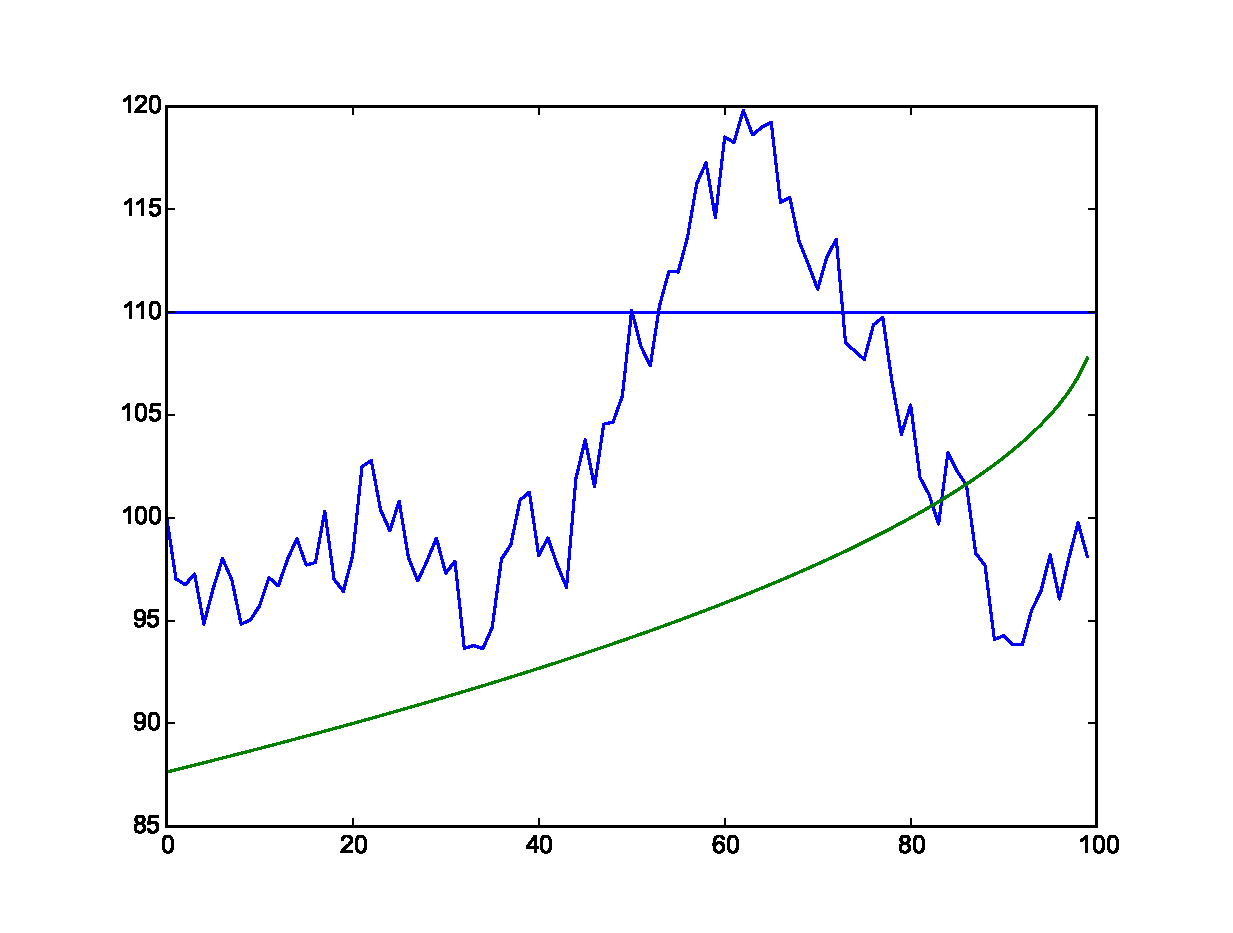
\includegraphics[width=0.7\textwidth]{random_process_with_excercise_boundary}
\caption{Граница исполнения для Американского опциона пут с функцией выплат $\left(K-S(t)\right)^+$ (форма границы --- примерная, точная форма неизвестна). Опцион исполняется, как только цена актива впервые достигает границы. Горизонтальная линия --- цена страйк опционного контракта. Пунктирной линией отмечен момент оптимального исполнения опциона.}
\label{fig:excercise_boundary}
\end{figure}

\paragraph{Метод стохастической сетки}
Метод стохастической сетки решает задачу динамического программирования \eqref{eq:common_recursive_statement} с помощью генерирования случайных траекторий состояния базового актива. Сетку, получающуюся при назначении всех вершин предыдущего поколения родительскими вершинами для всех вершин следующего поколения, можно увидеть на рис. \ref{fig:stohastic_mesh}.
\begin{figure}[htpb]
\centering
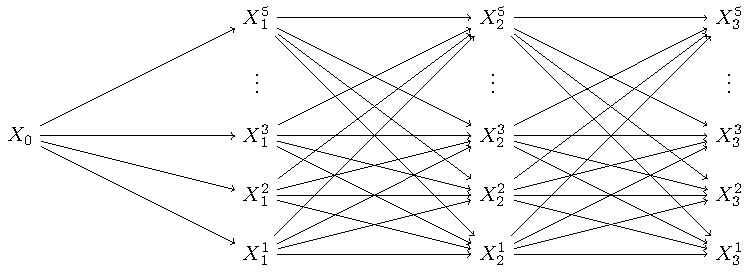
\includegraphics[width=0.7\textwidth]{stohastic_mesh_vector}
\caption{Сетка состояний базового актива при использовании метода стохастической сетки}
\label{fig:stohastic_mesh}
\end{figure}

Количество узлов в сетке ограничено $mn$, где $m$ ---  число дат исполнения опциона, $n$ --- число промоделированных траекторий. Неоднозначным остаётся лишь выбор весов, присвиваемых дугам сетки.

Все вышеописанные методы подробно рассмотрены в \cite{Glasserman2004}.

Также существуют некоторые аналитические формы приближённых оценок стоимости Американского опциона (см. \cite{Haug2007}, глава 3, и последующие ссылки), но они накладывают более жёсткие ограничения на сущность базового актива.

В следующей главе подробно рассматривается ещё один имитационный метод оценки: метод случайных деревьев, являющийся объектом исследования этой работы. Обладая некоторыми существенными недостатками, он, тем не менее, представляет интерес для исследования из-за потенциальной возможности обощения на более широкий класс задач.
